\documentclass[spanish]{article}
\usepackage[a4paper, left=1in, right=1in, top=1in, bottom=1in]{geometry}
                                % for page size and margin settings
\usepackage{graphicx}		    % for insert images
\usepackage[es-tabla]{babel} 	% for spanish titles
\usepackage[a4paper, left=1in, right=1in, top=1in, bottom=1in]{geometry} 
								% for page size and margin settings
\usepackage{mathtools}          % for greek math symbol formatting
\usepackage{enumitem}           % for control of 'enumerate' numbering
\usepackage{listings}           % for control of 'itemize' spacing
\usepackage{indentfirst}		% package to make first paragraph always indented
\usepackage{hyperref}           % page numbers and '\ref's become clickable
\usepackage{bm}					% for bold maths
\usepackage{setspace}			% for setting interline spacing
\usepackage{amsmath}			% for matrices
\usepackage{tikz} 				% for graphs
\usepackage{multirow}			% for tables
\usepackage{float}				% to manually select placement of tables

\usetikzlibrary{babel}		    % for draw arrows in tikz using babel spanish
\renewcommand{\baselinestretch}{1.5}
\bibliographystyle{ieeetr}
\numberwithin{figure}{subsection}
\numberwithin{equation}{subsection}
\numberwithin{table}{subsection}

% TITLE VARIABLES 

\def\thesistitle{Modelos longitudinales con covariables que varían en el tiempo}
\def\thesisauthorfirst{\textbf{Esteban Cometto}}
\def\thesissupervisorfirst{Noelia Castellana}
\def\thesissupervisorsecond{Cecilia Rapelli}
\def\thesisdate{\today}

%% OTHER USEFUL VARIABLES 

\def\npatients{560}
\def\fullcovname{adherencia al tratamiento farmacológico}
\def\covname{\textit{adherencia}}
\def\cvt{covariable que varía en el tiempo}
\def\xseqj{$X_{i1}, ..., X_{ij}$}
\def\xseqn{$X_{i1}, ..., X_{in_i}$}
\def\xseqjminus{$X_{i1}, ..., X_{ij-1}$}
\def\yseqj{$Y_{i1}, ..., Y_{ij}$}
\def\yseqn{$Y_{i1}, ..., Y_{in_i}$}
\def\yseqjminus{$Y_{i1}, ..., Y_{ij-1}$}

%% FOR PDF METADATA
\title{\thesistitle}
\author{\thesisauthorfirst\space\thesisauthorsecond}
\date{\thesisdate}

\begin{document}

\begin{titlepage}
    \newcommand{\HRule}{\rule{\linewidth}{0.5mm}}
	\center
	\textsc{\Large Universidad Nacional de Rosario}\\[.7cm]
	
\includegraphics[width=25mm]{img/fceye-unr.png}\\[.5cm]
	\textsc{Facultad de Ciencias Económicas y Estadística}\\[0.5cm]
	\textsc{Anteproyecto de Tesina}
	
	\HRule \\[0.4cm]
	{ \huge \bfseries \thesistitle}\\[0.1cm]
	\HRule \\[.5cm]
	
	\begin{minipage}{0.6\textwidth}
	\large
	\textit{Autor:}	\thesisauthorfirst
	\end{minipage}
	\\[.6cm]
	\begin{minipage}{0.6\textwidth}
	\textit{Directora:} 	\thesissupervisorfirst \\[.2cm]
	\textit{Codirectora:} 	\thesissupervisorsecond
	\end{minipage}
	\\[4cm]
	\vfill
	{\large \thesisdate}\\
	\clearpage
\end{titlepage}

\newpage
\tableofcontents

\newpage
\section{Introducción}

%% Tesis mara catalano, silvia camats y redacción mia

Los datos longitudinales están conformados por mediciones repetidas de una
misma variable realizadas a la misma unidad. Estas mediciones surgen de
observar unidades en diferentes ocasiones, es decir en diferentes momentos o
condiciones experimentales.

Dado que las mediciones repetidas son obtenidas de la misma unidad, los datos
longitudinales están agrupados. Las observaciones dentro de un mismo
agrupamiento generalmente están correlacionadas positivamente. Por lo tanto,
los supuestos usuales acerca de la independencia entre las respuestas de cada
unidad y la homogeneidad de variancias frecuentemente no son válidos

El objetivo principal de estos estudios es estudiar los cambios en el tiempo y
los factores que influencian el cambio.

Las ocasiones en las que se registran las mediciones repetidas no
necesariamente serán iguales para todos los individuos, por lo tanto se pueden
obtener tanto estudios balanceados (todos los individuos tienen el mismo número
de mediciones durante un conjunto de ocasiones comunes) como desbalanceados (la
secuencia de tiempos de observaciones no es igual para todos los individuos).
Otra característica de estos datos es que en ocasiones se pueden obtener
valores perdidos, obteniendo datos incompletos aunque se cuente con un estudio
balanceado.

Los modelos mixtos permiten ajustar datos con estas particularidades, donde la
respuesta es modelada por una parte sistemática que está formada por una
combinación de características poblacionales que son compartidas por todas las
unidades (efectos fijos), y una parte aleatoria que está constituida por
efectos específicos de cada unidad (efectos aleatorios) y por el error
aleatorio. Estos modelos permiten, además, hacer predicciones del perfil de una
unidad específica. La selección de la estructura de covariancia apropiada
produce estimadores más eficientes y consecuentemente, pruebas estadísticas más
robustas para los efectos de interés

%% Chapter lalonde

Las covariables en los estudios longitudinales se pueden clasificar en dos
categorias: fijas y variables en el tiempo. Las diferencias entre estos tipos
de covariables pueden llevar a diferentes intereses de investigación,
diferentes tipos de análisis y diferentes conclusiones.

Las covariables fijas son variables independientes que no tienen variación
intra-sujeto, lo que significa que el valor de la covariable no cambia para un
individuo determinado en el estudio longitudinal. Este tipo de covariable se
puede usar para realizar comparaciones entre poblaciones y describir diferentes
tendencias en el tiempo, pero no permite una relación dinámica entre la
covariable y la respuesta.

Las covariables variables en el tiempo (CVT) son variables independientes que
contienen ambas variaciones, intra y entre sujeto, lo que significa que el
valor de la covariable cambia para un individuo determinado a lo largo del
tiempo y además puede cambiar para diferentes sujetos. Una CVT se puede usar
para hacer comparaciones entre poblaciones, describir tendencias en el tiempo y
también la relación dinámica entre la CVT y la respuesta

Se puede ver que las CVT permiten diferentes tipos de relaciones y conclusiones
que las covariables fijas. Por ejemplo, una CVT puede estar involucrada en
efectos acumulados para diferentes valores a través del tiempo (Fitzmaurice y
Lard 1995). Además, ciertas CVT transmiten diferente información que otras. Por
ejemplo, covariables como la edad pueden cambiar a través del tiempo, pero
cambian de manera predecible. Por otro lado, covariables como la precipitación
diaria pueden cambiar a través del tiempo pero no pueden ser predecidas. En
esos casos es importante considerar las relaciones entre la CVT y la respuesta
a través del tiempo.

%% Redacción mia

En el presente informe se cuenta con un programa de atención y control de
pacientes hipertensos iniciado en el año 2014 en Rosario que realiza un
seguimiento exhaustivo de \npatients{} pacientes. Este programa contempla:
efectores no médicos supervisados, tratamiento farmacológico genérico para la
hipertensión y utilización de un algoritmo terapéutico sistematizado. En cada
visita se registran tantocaracterísticas de los pacientes, del tratamiento y de
los valores de la tensión arterial. En particular, se desea evaluar si la
adherencia al tratamiento farmacológico influye en los valores de la tensión
arterial sistólica a lo largo del seguimiento. Como la variable
“\fullcovname{}” es una CVT estocástica se evaluaran diferentes enfoques para
incluirla en un modelo longitudinal que pueda explicar el cambio en la tensión
arterial sistólica media a lo largo del tiempo.

Un aspecto a tener en cuenta en este trabajo es que, si bien contamos con mucha
otra información para obtener modelos que describan de mejor manera el
comportamiento de la TAS, nos centraremos en modelos más simples con respecto a
las covariables fijas con el fin de no perder de vista la relación entre la
variable respuesta y la CVT.

\newpage
\section{Objetivos}

\subsection{Objetivo Principal}

Profundizar en el estudio de propuestas metodológicas para utilizar la
información obtenida de la \cvt{} dentro de un modelo mixto.

\subsection{Objetivos Específicos}

\begin{itemize}
	\item Específicar distintos tipos de CVT
	\item Transformaciones a realizar sobre la CVT antes de incluirla al
	modelo, incluyendo conversión a covariable fija
	\item Consideraciones sobre interpretación de los parámetros sobre las CVT
	\item Indagar sobre feedback entre la CVT y la variable respuesta
\end{itemize}

\newpage
\section{Metodología}

\subsection{Los Datos Longitudinales}

Los datos longitudinales están conformados por mediciones repetidas de una
misma variable realizadas a la misma unidad. Estas mediciones surgen de
observar unidades en diferentes ocasiones, es decir en diferentes momentos o
condiciones experimentales.

Dado que las mediciones repetidas son obtenidas de la misma unidad, los datos
longitudinales están agrupados. Las observaciones dentro de un mismo
agrupamiento generalmente están correlacionadas positivamente.

El objetivo principal de estos estudios es estudiar los cambios en el tiempo y
los factores que influencian el cambio. 

Las ocasiones en las que se registran las mediciones repetidas no
necesariamente serán iguales para todos los individuos, por lo tanto se pueden
obtener tanto estudios balanceados (todos los individuos tienen el mismo número
de mediciones durante un conjunto de ocasiones comunes) como desbalanceados (la
secuencia de tiempos de observaciones no es igual para todos los individuos).
Otra característica de estos datos es que en ocasiones se pueden obtener
valores perdidos, obteniendo datos incompletos aunque se cuente con un estudio
balanceado.

Con el fin de simplificar la notación, se asumirá que los tiempos de medición
son los mismos para todas las unidades y que no hay datos faltantes.

Se obtiene una muestra de $N$ unidades cada una con $n$ mediciones repetidas de
la variable en estudio, observadas en los tiempos $t_1, t_2, ..., t_n$, siendo
entonces el número total de observaciones $N^*=Nn$. Se le llama $Y_{ij}$ a la
medición sobre la unidad $i$ en la ocasión $j$, con $i=1, ..., N; j=1, ..., n$

Asociadas a cada unidad se observan las covariables $X_{ij}$, de las cuales
existen dos tipos: variables en el tiempo (estocásticas) e invariables en el
tiempo (estacionarias)

Existen estudios empíricos que llevan a pensar que existen tres fuentes
potenciales de variabilidad que influyen sobre la correlación entre medidas
repetidas:

\begin{itemize}
	\item \textit{Heterogeneidad entre las unidades:} Refleja la propensión
	natural de las unidades a responder. Los individuos tienen diferentes
	reacciones frente a los mismos estímulos.
	\item \textit{Variación biológica intra-unidad:} Se piensa que la secuencia
	de medidas repetidas de una unidad tiene un comportamiento determinado, que
	produce que las mediciones más cercanas sean más parecidas.
	\item \textit{Error de medición:} Surge debido a los errores de medida, se
	puede disminuir usando instrumentos de medición más precisos
\end{itemize}

Estas tres fuentes de variación pueden clasificarse en \textit{``variabilidad
entre''}, es decir, la variación entre las unidades (heterogeneidad entre
unidades) y \textit{``variabilidad intra''}, es decir, la variación entre las
mediciones de las misma unidad (variación biológica intra-unidad y error de
medición)

Dado que, como se mencionó anteriormente, las mediciones están correlacionadas
sí, si se utilizaran las técnicas habituales basadas en la independencia entre
mediciones, los errores estándares nominales van a ser incorrectos, lo cual nos
llevaría a inferencias incorrectas sobre los parámetros del modelo. En base a
esto, surgen técnicas que consideran esa correlación modelando los datos
considerando la modelación de dos estructuras: la parte media y la estructura
de covariancia.

\subsection{Análisis exploratorio}

Antes de ajustar algún modelo, lo primero siempre es realizar un análisis
exploratorio para estudiar cómo se comportan los datos. A continuación se
presentan técnicas gráficas para cada estructura.

\textit{Evaluación de la parte media}

\begin{itemize}
	\item \textit{Perfil individual:} Consiste en un gráfico de dispersión en
	el cual se representan las respuestas vs las ocasiones. Cada respuesta
	tiene un punto y se une con un segmento los puntos de la misma unidad.
	Sirven para detectar si hay mucha variabilidad entre y dentro de las
	unidades y si hay valores atípicos.
	\item \textit{Perfiles promedio por grupo:} En general son más
	informativos. Para cada tiempo calculamos un promedio para cada grupo y
	luego se unen los puntos. Permiten ver la tendencia de las variables a
	través de las ocasiones. Se superponen en un mismo gráfico los perfiles
	promedio de cada grupo
\end{itemize}

\textit{Evaluación de la estructura de covariancia}

\begin{itemize}
	\item \textit{Matriz de diagrama de dispersión:} Para cada par de ocasiones
	se grafican los valores esperados de la respuesta y todos estos gráficos se
	acomodan dentro de una matriz. En general se utiliza cuando las ocasiones
	son las mismas para todas las unidades.
	\item \textit{Gráfico de Draftman:} Es similar al gráfico anterior pero
	utilizando variables estandarizadas. La utilización de la variable
	respuesta estandarizada ayuda a eliminar la variabilidad de los datos
	asociada con diferencias en las medias y variancias en el tiempo,
	permitiendo visualizar más claramente el patrón de correlación.
	\item \textit{Gráfico PRISM (Partial Regression on Intervenors Scatterplot
	Matrix):} Utilizando la variable estandarizada se crea una matriz de
	gráficos de dispersión. En la primera diagonal se encuentran gráficos de
	dispersión entre la variable respuesta en los tiempos $t_j$ y $t_{j+1}$.
	Luego, en la k-ésima diagonal, se obtienen gráficos de regresión parcial de
	las respuestas en los tiempos $t_j$ y $t_{j+k}$, ajustadas por las
	respuestas en los tiempos intermedios. Estos gráficos permiten ver con
	mayor claridad ciertos tipos de estructuras seriales que se dan entre las
	medidas repetidas.
	\item \textit{Correlograma:} Representa las características que existen
	entre las respuestas de los individuos de cada grupo en tiempos que están
	separados una cantidad de periodos. Permite analizar cómo evoluciona la
	correlación a medida que aumenta el número de rezagos.
	\item \textit{Semivariograma:} Cuando los datos están desbalanceados, el
	semivariograma permite distinguir las 3 fuentes de variabilidad. Después de
	haber estimado un modelo, el mismo permite confirmar si la estructura de
	correlación es adecuada. El semivariograma se define como una función:
	\[ \gamma(u) = \frac{1}{2} E[(\varepsilon _{ij} - \varepsilon_{ij'})^2] \]
	\[ u_{ijj'} = |t_{ij} - t_{ij'}| \]
	\[ \widehat{\gamma(u)} = v_{ijj'} = \frac{1}{2} (r_{ij} - r_{ij'}) \] donde
	$r_{ij}$ y $r_{ij'}$ son los residuos estandarizados obtenidos después de
	ajustar un modelo de regresión considerando las observaciones
	independientes.

	Se va a obtener un gráfico donde la variabilidad total va a estar dividida
	en 3 partes. Si la curva no empieza en cero significa que hay error de
	medición, si tiene pendiente quiere decir que hay un error debido a una
	causa biológica (correlación serial) y si la misma no llega a la variancia
	total significa que se debe explicar la variabilidad entre.
\end{itemize}

\subsection{Modelo lineal general para datos longitudinales}

Si se piensa que existe una tendencia en el tiempo de las respuestas, y esta
tendencia se puede expresar como una función, se puede escribir o representar a
las medidas repetidas de una unidad en un vector $Y_i$. Entonces, un modelo
lineal para representar la evolución en el tiempo va a ser:
\[ Y_i = X_i\beta + \varepsilon_i; \quad i = 1, ..., N; \quad Y_i = (Y_{i1},
Y_{i2}, ..., Y_{in_{i}})' \] Donde:

\begin{itemize}
	\item $Y_{ij}$: respuesta obtenida de la i-ésima unidad en la ocasión
	$t_{ij}$.
	\item $X_i$: matriz de diseño de la i-ésima unidad, de dimensión $(n_i*p)$
	\item $\beta $: vector de parámetros de dimensión $(p*1)$
	\item $\varepsilon_i$: vector de errores aleatorios de la i-ésima unidad,
	de dimensión $(n_i*1)$, este mismo representa todas las fuentes de
	variabilidad de los datos longitudinales
	\[ \varepsilon_i \sim N_{n_i}(0, \varSigma_i(\theta )) \]
	\item $\theta$: vector de parámetros desconocidos de covariancia, de
	dimensión $(q*1)$
\end{itemize}

\subsection{Modelación de la estructura de covariancia}

Al tenerse tantos parámetros de variancia $(n)$ y covariancia $n(n-1)/2$ para
estimar, se proponen modelos específicos para la estructura de correlación. Se
trata de elegir una estructura que no tenga tantos parámetros. Sin embargo, se
debe tener cuidado de no seleccionar estructuras demasiado parcas con las que
se pierda información.

La matriz de covariancia de cada unidad va a ser función de $\theta$. El número
de parámetros de este vector depende de la estructura de la matriz.

A continuación se mencionan algunas estructuras que se pueden utilizar, se
llamará $R$ a la matriz de correlaciones

\subsubsection{Arbitraria o no estructurada (datos balanceados)}

Considera variancias y covariancias distintas entre las mediciones repetidas.
Siendo $\sigma_{jj'} = Cov(Y_{ij}Y_{ij'})$ se expresa como:
\[
\varSigma = 
\begin{bmatrix}
	\sigma_{1}^2 & \sigma_{12}  & \dots  & \sigma_{1n} \\
	\sigma_{21}  & \sigma_{2}^2 & \dots  & \sigma_{2n} \\
	\vdots 		 & \vdots	    & \ddots & \vdots	   \\
	\sigma_{n1}  & \sigma_{n2}  & \dots  & \sigma_{n}^2
\end{bmatrix}
\]
La ausencia de restricciones hace que haya que estimar una gran cantidad de
parámetros

\subsubsection{Simetria compuesta (datos balanceados o no balanceados)}

La correlación entre pares de observaciones es la misma, sin importar la
cantidad de rezagos entre ellas,
$Corr(Y_{ij}, Y_{ik}) = \rho $ para todo $j \neq k$
\[
R_i =
\begin{bmatrix}
	1      & \rho   & \dots  & \rho \\
	\rho   & 1      & \dots  & \rho \\
	\vdots & \vdots	& \ddots & \vdots \\
	\rho   & \rho   & \dots  & 1
\end{bmatrix}
\]

\subsubsection{Toeplitz (datos equiespaciados)}
Se plantea para que cualquier par de respuestas que estén igualmente separadas
en el tiempo la correlación es la misma, $Corr(Y_{ij},Y_{ij+k}) = \rho_{k}$
para todo $j$ y $k$.
\[
R_i =
\begin{bmatrix}
	1      & \rho_1 	& \dots  & \rho_n \\
	\rho_1 & 1     		& \dots  & \rho_{n-1} \\
	\vdots & \vdots		& \ddots & \vdots \\
	\rho_n & \rho_{n-1} & \dots  & 1
\end{bmatrix}
\]

\subsubsection{Autorregresiva de primer orden (datos equiespaciados)}
Es un caso especial de la estructura anterior, en la que
$Corr(Y_{ij}, Y_{ij+k}) = \rho^k$. Esta estructura asume que la correlación
entre medidas repetidas disminuye a medida que aumenta el número de rezagos
entre ellas.
\[
R_i =
\begin{bmatrix}
	1      & \rho 	    & \dots  & \rho^n \\
	\rho   & 1     		& \dots  & \rho^{n-1} \\
	\vdots & \vdots		& \ddots & \vdots \\
	\rho^n & \rho^{n-1} & \dots  & 1
\end{bmatrix}
\]

\subsubsection{Markov (datos no equiespaciados)}

Es una generalización de la estructura autorregresiva para mediciones no
equiespaciadas. $Corr(Y_{ij}, Y_{ij'}) = \rho^{d_{jj'}}$, donde
$d_{jj'} = |t_{ij} - t_{ij'}|$ para todo $j \neq j'$.
\[
R_i =
\begin{bmatrix}
	1      		  & \rho^{d_{12}} & \dots  & \rho^{d_{1n}} \\
	\rho^{d_{21}} & 1     		  & \dots  & \rho^{n-1} \\
	\vdots 		  & \vdots		  & \ddots & \vdots \\
	\rho^n 		  & \rho^{n-1}    & \dots  & 1
\end{bmatrix}
\]

\subsection{Modelos lineales mixtos}

En estos modelos, cada unidad tiene una trayectoria individual caracterizada
por parámetros y un subconjunto de esos parámetros ahora se consideran
aleatorios. La respuesta media es modelada como una combinación de
características poblacionales que son comunes a todos los individuos (efectos
fijos) y efectos específicos de la unidad que son únicos de ella (efectos
aleatorios).

Se consideran las dos fuentes de variación (intra y entre) presentes en los
datos longitudinales. Entonces, este modelo va a ser similar al modelo lineal
general con respecto a la parte media del mismo, pero se va a diferenciar en
cuanto a la estructura de covariancia.

El modelo lineal mixto para la unidad $i$ se puede expresar en forma matricial
como:

\[ Y_i = X_i\beta + Z_ib_i + \varepsilon_i; \quad i = 1, ..., N;
\quad Y_i = (Y_{i1}, Y_{i2}, ... Y_{in_{i}})' \]

Donde:

\begin{itemize}
	\item $Y_i$: Vector de la variable respuesta de la i-ésima unidad, de
	dimensión $(n_i*1)$
	\item $X_i$: Matriz de diseño de la i-ésima unidad, que caracteriza la
	parte sistemática de la respuesta, de dimensión $(n_i*p)$
	\item $\beta$: Vector de parámetros de dimensión $(p*1)$
	\item $Z_i$: Matriz de diseño de la i-ésima unidad, que caracteriza la
	parte aleatoria de la respuesta, de dimensión $(n_i*k)$
	\item $b_i$: Vector de efectos aleatorios de la i-ésima unidad, de
	dimensión $(k*1)$
	\item $\varepsilon_i$: Vector de errores aleatorios de la i-ésima unidad,
	de dimensión $(n_i*1)$
\end{itemize}

$\varepsilon_i$ y $b_i$ son independientes.

\[ \varepsilon_i \sim N_{n_i}(0, R_i) \]
\[ b_i \sim N_k(0, D_i) \]

Las matrices $D_i$ y $R_i$ contienen las variancias y covariancias de los
elementos de los vectores $b_i$ y $\varepsilon_i$ respectivamente. A partir de
este modelo se obtiene:

\begin{itemize}
	\item $E(y_i/b_i) = X_i\beta + Z_ib_i$ (media condicional o específica de
	la i-ésima unidad)
	\item $E(Y_i) = X_i\beta$ (media marginal)
	\item $Cov(Y_i/b_i) = R_i$ (variancia condicional)
	\item $Cov(Y_i) = Z_iD_iZ'_i + R_i = \varSigma_i$ (variancia marginal)
\end{itemize}

Generalmente, la matriz $D_i$ adopta una estructura de covariancia arbitraria,
mientras que la matriz $R_i$ adopta cualquiera de las vistas anteriormente

\subsection{Estimación de los parámetros del modelo}

Bajo el supuesto de que $\varepsilon_i$ y $b_i$ se distribuyen normalmente se
pueden usar métodos de estimación basados en la teoría de máxima verosimilitud,
cuya idea es asignar a los parámetros el valor más probable en base a los datos
que fueron observados. Se usarán para estimar los parámetros de la parte media
y los de las estructuras de covariancia los métodos de máxima verosimilitud
(ML) y máxima verosimilitud restringida (REML) respectivamente

\subsubsection{Método de máxima verosimilitud (ML)}

Bajo el supuesto de que $Y_i \sim N_{n_i}(X_i\beta, \varSigma_i)$ y las $Y_i$
son independientes entre sí, se obtiene la siguiente función de
log-verosimilitud:

\begin{equation}
\label{ML}
	l = -\frac{1}{2} \sum_{i=1}^{N}n_i ln(2\pi) - \frac{1}{2}ln|\varSigma_i| -
	\frac{1}{2} \sum_{i=1}^{N} [(Y_i - X_i\beta)'
	\varSigma_i^{-1} (Y_i - X_i\beta)]
\end{equation}

Siendo $\varSigma_i$ función del vector $\theta$ que contiene los parámetros de
covariancia.

La ecuación anterior se debe derivar con respecto a $\beta$ y $\theta$ y luego
debe igualarse a cero, de esta manera se obtienen sus estimadores. Cuando
$\theta$ es desconocido (lo que generalmente sucede) se obtiene una ecuación no
lineal, por lo que no se puede obtener una expresión explícita de
$\hat{\theta}$, para encontrar su solución se recurren a algoritmos numéricos.
El estimador del vector $\beta$ resulta:

\[ \hat{\beta} = (\sum_{i=1}^{N} X_i'\hat{\varSigma_i}^{-1}X_i)^{-1}
\sum_{i=1}^{N} X'_i\hat{\varSigma_i}^{-1}Y_i \]

El estimador $\hat{\beta}$ resulta insesgado de $\beta$. Cuando $\theta$ es
conocido se conoce la distribución exacta del estimador. Sin embargo, cuando es
desconocido, no se puede calcular de manera exacta la matriz de covariancias de
$\hat{\beta}$. Si el número de unidades es grande se puede demostrar que
asintóticamente:

\[ \hat{\beta} \sim N_p(\beta, V_{\beta}) \quad donde \quad V_{\beta} =
(\sum_{i=1}^{N} X'_i\hat{\varSigma_i}^{-1}X_i)^{-1} \]

\subsubsection{Método de máxima verosimilitud restringida (REML)}

El inconveniente que posee el método de MV es que los parámetros de covariancia
resultan sesgados. Es decir, a pesar de que la estimación de $\beta$ resulta
insesgada, no pasa lo mismo con $\theta$. Si el tamaño de muestra es chico, los
parámetros que representan las variancias van a ser demasiado pequeños, dando
así una visión muy optimista de la variabilidad de las mediciones, es decir, se
subestiman los parámetros de covariancia. El sesgo se debe a que en la
estimación MV no se tiene en cuenta que $\beta$ es estimado a partir de los
datos.

El método REML separa la parte de los datos usada para estimar $\beta$ de
aquella usada para estimar los parámetros de $\varSigma_i$, la función de
log-verosimilitud restringida que se propone es:

\begin{equation}
\label{REML}
	l^* = -\frac{1}{2} \sum_{i=1}^{N}n_i ln(2\pi) - \frac{1}{2}ln|\varSigma_i| -
	\frac{1}{2} \sum_{i=1}^{N} [(Y_i - X_i\beta)'
	\varSigma_i^{-1} (Y_i - X_i\beta)] -
	- \frac{1}{2} ln |\sum_{i=1}^{N} X'_i \hat{\varSigma_i^{-1} X_i}|
\end{equation}

Maximizando esta funcion con respecto a $\beta$ y $\theta$ se obtiene:

\[ \hat{\beta} = (\sum_{i=1}^{N} X'_i \hat{\varSigma}_i^{-1} X_i)^{-1}
\sum_{i=1}^{N} X'_i \hat{\varSigma}_i^{-1} Y_i\]

Donde $\hat{\varSigma}_i$ es el estimador REML de ${\varSigma_i}$

\subsection{Pruebas de hipótesis}

Generalmente, la inferencia en estos modelos se centra en los parámetros de la
parte media. Es decir, en combinaciones lineales de los parámetros de $\beta$.
La hipótesis lineal general para los test se plantea construyendo dichas
combinaciones a través de $L'\beta$, siendo $L'$ una matriz de dimensión
$(r*p)$.

El estimador de $L'\beta$ resulta $L'\hat{\beta}$ y asintóticamente su
distribución muestral es aproximadamente:

\[ L'\beta \sim N_p(L'\beta, L'V_{\beta}L) \]

Para probar las hipótesis se proponen dos métodos basados en la función de
verosimilitud:

\subsubsection{Test de Wald}

Se plantean las hipótesis:

\[ H_0) L'\beta = 0 \quad H_1) L'\beta \neq 0 \]

La estadística de prueba resulta:

\[ W = (L'\hat{\beta})' (L'\hat{V}_{\beta}L)^{-1} (L'\hat{\beta}) \]

Donde $W$ se distribuye aproximadamente como $\chi_r^2$.

Este test provee inferencias válidas cuando el $N$ es grande, ya que utiliza la
aproximación asintótica a la distribución Normal. Si el $N$ es chico se propone
reemplazar la distribución de la chi-cuadrado por una $F$ de Snedecor. El
problema con el uso de esta estadística es que no se conocen los grados de
libertad del denominador y deben ser calculados con los datos. 

%Algunos métodos para estimar los grados de libertad son: Contaiment,
%Within-Between, Satterthwaite y Kenward y Roger, entre otros
%(\textit{Fitzmaurice et al., 2004})

\subsubsection{Test de cociente de verosimilitud}

Se basa en la teoría asintótica y va a suplir las dificultades del test de
Wald. El test se obtiene comparando las verosimilitudes de dos modelos, uno de
los cuales incorpora la restricción $L'\beta = 0$ (modelo reducido) y el otro
no tiene restricciones (mdoelo completo). Estos dos modelos están anidados, ya
que el modelo reducido es un caso particular del modelo completo.

Al igual que anteriormente, se plantean las hipótesis:

\[ H_0) L'\beta = 0 \quad H_1) L'\beta \neq 0 \]

La función de log-verosimilitud maximizada del modelo completo es:

\[ -\frac{1}{2} \sum_{i=1}^{N}n_i ln(2\pi) - \frac{1}{2}ln|\varSigma_i| -
\frac{1}{2} \sum_{i=1}^{N} [(Y_i -
X_i\hat{\beta})' \varSigma_i^{-1} (Y_i - X_i\hat{\beta})] \]

Y la del modelo reducido es:

\[ -\frac{1}{2} \sum_{i=1}^{N}n_i ln(2\pi) - \frac{1}{2}ln|\varSigma_i| -
\frac{1}{2} \sum_{i=1}^{N} [(Y_i - X_i\beta_0)' \varSigma_i^{-1}
(Y_i - X_i\beta_0)] \]

Donde $\beta_0$ es el vector de parámetros resultante de haber impuesto
$L'\beta = 0$.

Si el $N$ es grande, la distribución muestral aproximada de la estadística es:

\[ G^2 = -2 (\hat{l}_{red} - \hat{l}_{comp}) \sim \chi_v^2 \]

Donde $v$ es el número de parámetros del modelo completo menos el número de
parámetros del modelo reducido

Si lo que se quiere comparar mediante este test es la estructura media de dos
modelos, se recomienda estimar los parámetros mediante el método ML. En cambio,
si lo que se desea comparar son patrones de covariancia anidados entre dos
modelos se recomienda estimar los parámetros con el método REML.

Cuando se desea hacer inferencia sobre las componentes de variancia (por
ejemplo, postular que una variancia es nula), la diferencia entre los dos
modelos va a ser de $k+1$ parámetros (1 de variancia y $k$ de covariancia). Si
sucede esto, la distribución de la estadística $G^2$ ya no será una
chi-cuadrado común, si no que será una mezcla entre dos chi-cuadrado, una de
$k$ grados de libertad y otra de $k+1$ grados de libertad.

% Si bien hay tablas para esta estadística, se recomienda en general utilizar
% en vez de un nivel de significación del 5%, uno del 10%, para no tener
% problemas de elegir un modelo demasiado simple

\subsection{Elección entre modelos de covariancia}

Cuando los modelos no están anidados, como sucede generalmente cuando se
plantean modelos con distintas estructuras de covariancia, no se puede usar el
método del cociente de verosimilitud para compararlos.

Como en la matriz de covariancia siempre intervienen los residuos, y en ellos
aparecen los parámetros de la parte media del modelo, para asegurarse que la
parte media esté bien especificada se elige un modelo maximal (modelo con todos
los parámetros que queremos incorporar). Dado dicho modelo, se plantean
distintos modelos que se van a diferenciar únicamente en la estructura de la
matriz de covariancia.

Los enfoques que se proponen a continuación se basan en la comparación de
versiones penalizadas de las log-verosimilitudes de los modelos. Como es
conocido, a medida que se incorporan parámetros a los modelos, mayor va a ser
la verosimilitud. Para comparar modelos con distinto número de parámetros, se
penalizan a los mismos, surgiendo varios criterios A continuación se destacan
dos de estos:

\begin{itemize}
	\item \textit{Criterio de Akaike (AIC)}: $-2\hat{l} + 2p$
	\item \textit{Criterio bayesiano se Schwarz (BIC)}: $-2\hat{l} + p ln(N)$
\end{itemize}

Donde:

$\hat{l}$: log-verosimilitud maximizada del modelo

$p$: número de parámetros del modelo

El $BIC$ penaliza más la verosimilitud dando modelos más sencillos. El criterio
para seleccionar un modelo es aquel que minimice los valores de $AIC$ o $BIC$


\subsection{Predicción de los efectos aleatorios}

En muchas aplicaciones la inferencia está centrada solamente en los efectos
fijos. Estos parámetros se interpretan como los cambios de la respuesta media
en el tiempo, pero muchas veces se desea conocer además los perfiles
individuales, por lo que necesitamos conocer los valores de $b_i$. Como $b_i$
es una cantidad aleatoria se habla de predicción de $b_i$.

Llamando $c(Y_i)$ al predictor de los efectos aleatorios, se debe minimizar
$E[b_i - c(Y_i)]^2$. La función $c(Y_i)$ que hace que esa esperanza sea lo más
chica posible se llama esperanza condicional de $b_i$ dado $Y_i$ y se
simboliza:

\[ E(b_i/Y_i) = D_iZ'_i\varSigma_i^{-1} (Y_i - X_i\beta) \]

Esto se conoce como mejor predicción lineal insesgada (BLUP) y el BLUP empírico
(EBLUP) o estimador empírico de Bayes resulta:

\[ \hat{b_i} = \hat{D_i}Z'_i\hat{\varSigma_i}^{-1} (Y_i - X_i\hat{\beta}) \]

A través de esto se pueden conocer los perfiles individuales, siendo
$\hat{Y_i} = X_i\hat{\beta} + Z_i\hat{b_i}$,
operando algebraicamente se llega a la expresión:

\[ \hat{Y_i} = (\hat{R_i}\hat{\varSigma_i}^{-1}) X_i\beta + (I_n -
\hat{R_i}\hat{\varSigma_i}^{-1}) Y_i \]

Resulta que el perfil individual estimado es un promedio ponderado entre el
perfil de la respuesta media poblacional ($X_i\hat{\beta}$) y el perfil de la
respuesta observada en la unidad $i$ $(Y_i)$.

\subsection{Examen de residuos}

Como en todo análisis de datos en donde se utiliza un modelo estadístico, es
necesario realizar un estudio del cumplimiento de los supuestos del modelo
utilizando los gráficos de residuos.

El modelo lineal mixto para la unidad $i$ es:

\[ Y_i = X_i\beta + Z_i\beta + \varepsilon_i \]

Con $b_i$ y $\varepsilon_i$ independientes y
$\varepsilon \sim N_{n_i}(0, R_i)$, $b_i \sim N_k(0, D_i)$.

En los modelos lineales mixtos se va a distinguir entre tres tipos de residuos:

\subsubsection{Residuos marginales}

Se definen como la diferencia entre el vector de respuestas y su media marginal
estimada.

\[ r_{iM} = Y_i - \widehat{E(Y_i)} = Y_i - X_i\hat{\beta} \]

\subsubsection{Residuos condicionales}

Se definen como la diferencia entre el vector de respuestas y su media
condicional estimada.

\[ r_{iC} = Y_i - \widehat{E(Y_i/b_i)} = Y_i - X_i\hat{\beta} - Z_i\hat{b_i} \]

\subsubsection{Residuos de los efectos aleatorios}

\[ r_{iEA} = \widehat{E(Y_i/b_i)} - \widehat{E(Y_i)} = Z_i\hat{b_i} \]

Estos residuos así calculados reciben el nombre de residuos ordinarios, van a
estar correlacionados y sus variancias no van a ser necesariamente contrastes.
Para evitar este inconveniente es necesario realizar una estandarización de los
mismos:

\begin{itemize}
	\item Si se divide el residuo por $\sqrt{\widehat{Var(r_i)}}$ se obtienen
	los residuos estudentizados.
	\item Si se divide el residuo por $\sqrt{\widehat{Var(Y_i)}}$ se obtienen
	los residuos de Pearson.
\end{itemize}

Se define como residuo puro al residuo que depende de solo los componentes
fijos y del error que predice, y residuo confundido si además de depender de
las componentes fijas y del error que predicen están en función de otros
residuos.

% En el word hay una tabla que explica como usar cada residuo

%%%%%%%%%%%%%%%%%%%%%%%%%%%%%%%%%%%%%%%%%%%%%%%%%%
% DIGGLE
%%%%%%%%%%%%%%%%%%%%%%%%%%%%%%%%%%%%%%%%%%%%%%%%%%

\section{Covariables que varían en el tiempo}

En los estudios longitudinales, las variables independientes pueden ser
clasificadas en dos categorías: covariables fijas en el tiempo, es decir que no
varían en el tiempo (CNVT) o covariables que varían en el tiempo (CVT). La
diferencia entre ellas puede conducir a diferentes enfoques de análisis así
como también a diferentes conclusiones.

Las CNVT son variables independientes que no presentan variación intra-sujeto,
es decir, los valores de estas covariables no cambian a lo largo del estudio
para un individuo en particular. Por ejemplo, el sexo biológico de una persona
o el grupo de tratamiento.

Las CVT son variables independientes que incluyen tanto la variación
intra-sujeto y la variación entre-sujetos. Esto significa que, para un
individuo en particular, el valor de la covariable cambia a través del tiempo y
puede cambiar también entre diferentes individuos. Por ejemplo, valor de la
presión arterial o condición de fumar (si/no).

Tanto las CNVT y las CVT ueden ser utilizadas para realizar comparaciones entre
poblaciones y describir diferentes tendencias a lo largo del tiempo. Sin
embargo, sólo las CVT permiten describir una relación dinámica entre la
covariable y la variable respuesta.

\subsection{Covariables estocásticas y no estocásticas}

Las CVT no estocásticas son covariables que varían sistemáticamente a través
del tiempo pero son fijas por diseño del estudio o bien su valor puede
predecirse. En cambio, las CVT estocásticas son covariables que varían
aleatoriamente a través del tiempo, es decir, los valores en cualquier ocasión
no pueden ser estimados ya que son gobernados por un mecanismo aleatorio.
Ejemplos de las primeras son: tiempo desde la visita basal, edad, grupo de
tratamiento en los estudios cross-over. Ejemplos de las segunas son: valor del
colesterol, ingesta de alcohol (si/no), ingesta de grasas, etc.

\subsection{Covariables exógenas y endógenas}

Se dice que una CVT es exógena cuando los valores actuales y anteriores de la
respuesta en la ocasión $j (Y_{i1}, ..., Y_{ij})$, dados los valores actuales y
precedentes de la CVT $(X_{i1}, ..., X_{ij})$, no predicen el valor posterior
de $X_{ij+1}$. Más formalmente, una CVT es exógena cuando:

\begin{equation}
	\label{exogeneidad}
	f(X_{ij+1}|X_{i1}, ..., X_{ij}, Y_{i1}, ..., Y_{ij}) =
	f(X_{ij+1}|X_{i1}, ..., X_{ij})
\end{equation}

Y en consecuencia:

\begin{equation}
	\label{exogeneidad debil}
	E(Y_i|X_i) = E(Y_i|X_{i1}, ..., X_{in_i}) = E(Y_i|X_{i1}, ..., X_{ij})
\end{equation}

Esta definición implica que la respuesta en cualquier momento puede depender de
valores previos de la variable respuesta y de la CVT, pero será independiente
de todos los demás valores de la covariable. Por ejemplo, en un estudio
longitudinal en donde se evalúa si el nivel de polución en el aire está
asociado a la función pulmonar, es de esperar que el nivel de polución del aire
en una determinada ocasión dependa de los niveles observados previamente, pero
no se espera que dependa de los niveles de la función pulmonar observados
previamente en el sujeto.

Una CVT que no es exógena se define como endógena. Por ejemplo, cuando se
evalúa si la cantidad de actividad física está asociada al nivel de glicemia.
El nivel de actividad física en un determinado momento puede estar (o no)
asociado a niveles previos y también puede estar asociado a valores previos de
la glicemia (un paciente con valor de glicemia alto en una visita puede decidir
aumentar su nivel de actividad física para reducir este valor)

Es posible examinar empíricamente la suposición de que una CVT es exógena al
considerar modelos de regresión para la dependencia de $X_{ij}$ en
$Y_{i1}, ... Y_{ij-1}$ (o en alguna función conocida de
$Y_{i1}, ... Y_{ij-1}$) y $X_{i1}, ..., X_{ij-1}$ (o en alguna función conocida
de $X_{i1}, ... X_{ij-1}$). La ausencia de cualquier relación entre $X_ij$ y
$Y_{i1}, ... Y_{ij-1}$, dado el perfil de la covariable anterior
$X_{i1}, ..., X_{ij-1}$, proporciona soporte para la validez de la suposición
de que la CVT es exógena.

A los parámetros de regresión se les puede dar una interpretación causal sólo
cuando se puede asumir que las CVT son exógenas con respecto a la variable
respuesta.

\subsection{Otros tipos de CVT}

Trabajos más recientes han definido una nueva categorización de las CVT para
facilitar las interpretaciones y los métodos de estimación adecuados para el
modelo. Se pueden definir cuatro tipos de CVT relacionados con el grado de no
exogeneidad con respecto a la respuesta.

\subsubsection{CVT tipo I}

Se clasifica una CVT como de tipo I si satisface:

\begin{equation}
	\label{CVT tipo I}
	E(Y_{ij}|X_{i1}, ..., X_{in_i}) = E(Y_{ij}|X_{ij})
\end{equation}

En otras palabras, una CVT se considera de tipo I si la variable respuesta en
la j-ésima ocasión es independiente de todos los valores de la CVT en
diferentes momentos, aún de los previos a la ocasión. Variables que involucran
cambios predecibles en el tiempo son tratadas como CVT tipo I, por ejemplo la
edad o el momento de observación.

\subsubsection{CVT tipo II}

Una CVT se clasficia de tipo II si:

\begin{equation}
	\label{CVT tipo II}
	E(Y_{ij}|X_{i1}, ..., X_{in_i}) = E(Y_{ij}|X_{i1}, ..., X_{ij})
\end{equation}

Cabe destacar que la clase de covariables de tipo I es un subconjunto de la
clase de covariables de tipo II. Esta condición dice que el proceso de la CVT
$X_{ij+1}, ..., X_{in_i}$ no se ve afectado por la respuesta $Y_{ij}$.

En otras palabras, la variable respuesta en la j-ésima ocasión puede estar
asociada a valores previos de la CVT. Esta definición es similar pero no
equivalente a la definición de exogeneidad. Se puede demostrar que la
exogeneidad es suficiente es condición suficiente para que una CVT sea de tipo
II. Este tipo de CVT incluyen covariables que pueden tener una asociación
rezagada con la respuesta (los valores anteriores de la CVT pueden afectar a la
respuesta actual) pero los valores de la covariable en un momento determinado
no se verán afectados por los valores previos de la variable respuesta. Un
ejemplo de este tipo de CVT es el ``tratamiento farmacológico para la
hipertensión arterial'' con la variable respuesta ``presión arterial''.

\subsubsection{CVT tipo III}

Se clasifica a una CVT como de tipo III si no es de tipo II. No se asume
independencia entre la respuesta y la covariable, por lo tanto, uede existir un
\textit{feedback} entre ambas en donde los valores de la CVT pueden estar
afectados por valores previos de la variable respuesta. Un ejemplo de este tipo
de CVT es el ``tratamiento farmacológico para la hipertensión arterial'' con la
variable respuesta ``infarto de miocardio''. Mientras que es esperable que la
medicación impacte en la probabilidad de tener un infarto de miocardio, también
tener un infarto de miocardio puede impactar en el cambio del tratamiento
farmacológico.

\subsubsection{CVT tipo IV}

Una CVT se define como de tipo IV si:

\begin{equation}
	\label{CVT tipo IV}
	E(Y_{ij}|X_{i1}, ..., X_{in_i}) = E(Y_{ij}|X_{ij+1}, ..., X_{in_i})
\end{equation}

La CVT puede estar asociada con valores previos de la variable respuesta, pero
la variable respuesta no está asociada con valores previos de la covariable,
está sólo asociada con el valor observado de la covariable en la misma ocasión.
Un ejemplo de este tipo de CVT es ``presión arterial'' con la variable
respuesta ``peso''. En una determinada ocasión hay relación entre ambas
variables, es esperable que valores previos del peso impacten en la presión
arterial pero no al revés

\subsection{Covariables rezagadas}

En la mayoria de los casos, se suele utilizar solo la exposición que ocurre
antes del tiempo $t$ para predecir $Y_{it}$. Sin embargo, en algunas
aplicaciones, el historial completo de la covariable \xseqn{} está disponible y
es considerado como potencial predictor de la respuesta. En otras, solo un
pequeño subconjunto de las mediciones más recientes son usados, ya que se
supone que el efecto en la respuesta está concentrado en ellas. En cualquier
caso, el uso de más de una covariable rezagada puede llevar a predictores
altamente correlacionados, lo que lleva a preguntarse sobre la elección de
cuantos predictores rezagados utiliar y sobre la estructura de sus
coeficientes.

\subsubsection{Una sola covariable rezagada}

En algunas aplicaciones hay justificacion previa para considerar la covariable
en un solo rezago $k$ momentos antes de la medición de la respuesta. Por
ejemplo, muchos agentes farmacológicos son rápidamente limpiados del cuerpo,
por lo que sólo mantienen efectos por una corta duración. En este caso, si la
covariable es exógena, puede ajustarse el modelo mixto sin más consideraciones.
Lo más común es que se desconozca el valor $k$ apropiado y se consideren varias
opciones diferentes.

\subsubsection{Múltiples covaribales rezagadas}

La literatura de series de tiempo ha considerado modelos tanto para infinitos o
finitos rezagos de la covariable. Dado que los datos longitudinales son
tipicamente series de tiempo cortas, se puede proponer un modelo de menor
dimensión para los coeficientes de las covariables rezagadas. En los modelos
rezagados distribuidos, los coeficientes rezagados se asume que siguen una
función paramétrica suave de orden inferior. Por ejemplo, para un rezago finito
$L$, se puede usar un modelo polinomial de orden $p$, con $p < L$ para obtener
coeficientes de regresión suaves.

\[ Y_{it} = \beta_0 + \beta_1 X_{it-1} + \beta_2 X_{it-2} + ... +
\beta_L X_{it-L}, \]
\[ \beta_j = \gamma_0 + \gamma_1 j + \gamma_2 j^2 + ... + \gamma_p j^p \]

A pesar de que los modelos rezagados distribuidos permiten modelar
parsimoniosamente las covariables rezagadas múltiples, la especificación de del
número de rezagos, $L$, y el órden del modelo para el coeficiente, $p$, deben
ser consideradas. Ésto puede realizarse a través de tests para modelos
anidados, como el test del cociente de verosimilitud o el test de Wald.

\subsection{Confusores variables en el tiempo}

El análisis de regresión epidemiológica tradicional considera una clasificación
de variables que están relacionadas tanto con una exposición de interés como
con el resultado, ya sea como confusoras o intermedias. Una confusora se define
vagamente como una variable asociada tanto con la exposición de interés como
con la respuesta, y que, si se ignora en el análisis, conducirá a estimaciones
sesgadas del efecto de la exposición. Una variable intermedia es aquella que se
encuentra en la vía causal desde la exposición hasta el resultado y un análisis
no debe controlar dicha variable, ya que se pierde el efecto de la exposición
mediado por la variable intermedia.

Por ejemplo, en un estudio observacional de pacientes con hipertensión elevada,
podemos esperar determinar la magnitud del beneficio (o daño) atribuible a un
tratamiento en la supervivencia del paciente o medidas longitudinales como la
hipertensión en cierto momento. Sin embargo, podemos encontrar que la
hipertensión en el tiempo $t$ prediga tanto la hipertensión en momentos
posteriores como las opciones de tratamiento posteriores. En este caso, la
hipertensión en el momento $s < t$ es la variable de respuesta para las
opciones de tratamiento recibidas antes de $s$, pero también es un predictor y,
por lo tanto, un factor de confusión potencial para el tratamiento administrado
en momentos futuros, $t > s$.

\subsubsection{Feedback}

Para aclarar los problemas que surgen con las covariables dependientes del
tiempo, se consiidera un solo par de tiempos de estudio, $t = 0, 1$, con
medidas de exposición y respuesta $(X_{t-1}, Y_t)$. Sea $Y_t$ un indicador de
gravedad de la enfermedad o de los síntomas (1 = enfermedad/síntomas presentes,
0 = enfermedad/síntomas ausentes) y sea $X_t = 1$ si se administra tratamiento
y $0$ en caso contrario. Se supone que la exposición $X_{t-1}$ precede a $Y_t$
para $t = 1, 2$ y que $Y_t$ precede o se mide simultáneamente con $X_t$. La
figura 1 presenta un grafo que representa los modelos secuenciales
condicionales:

\begin{equation}
	\label{feedback_1}
	logit \ E(Y_1 / X_0 = x_0) = -0.5 - 0.5x_0,
\end{equation}
\begin{equation}
	\label{feedback_2}
	logit \ E(X_1 / Y_1 = y_1, X_0 = x_0) = -0.5 + 1y_1,
\end{equation}
\begin{equation}
	\label{feedback_3}
	logit \ E(Y_2 / H_1^X = h_1^X, Y_1 = y_1) = -1 + 1.5y_1 - 0.5x_1,
\end{equation}
\[ donde \ H_1^x = \{ X_0, X_1 \} \ y \ h_1^X = \{ x_0, x_1 \} \]

\begin{figure}[h]
\centering
\begin{tikzpicture}[node distance={15mm}, thick, main/.style = {draw, circle}]
	\node[main] (X0) {$X_0$};
	\node[main] (Y1) [right of=X0] {$Y_1$};
	\node[main] (X1) [below of=X0] {$X_1$};
	\node[main] (Y2) [below of=Y1] {$Y_2$};
	\draw [->] (X0) to (Y1);
	\draw [->] (Y1) to (X1);
	\draw [->] (Y1) to (Y2);
	\draw [->] (X1) to (Y2);
\end{tikzpicture}
\caption{Covariable variable en el tiempo, $X_{t-1}$, y respuesta $Y_t$.}
\end{figure}

Estos modelos especifican un efecto beneficioso del tratamiento $X_0$ sobre el
resultado en el momento 1 con una razón de odds logarítmica de -0,5 en el
modelo $[Y_1|X_0]$. Sin embargo, el segundo modelo especifica que el
tratamiento recibido en el momento 2 depende en gran medida del resultado en el
momento uno. Para $X_0 = 0$ o $X_0 = 1$, si los pacientes tienen una respuesta
inicial deficiente $(Y_1 = 1)$, es más probable que reciban tratamiento en el
momento 2 que si respondieran bien $(Y_1 = 0)$. Finalmente, la respuesta en el
segundo tiempo está fuertemente correlacionada con la respuesta inicial y está
influenciada por el tratamiento en el tiempo 2.

\begin{table}[H]
	\label{feedback_table}
	\caption{Recuentos esperados cuando se tratan inicialmente 500 sujetos,
	$X_0 = 1$, y 500 sujetos no reciben tratamiento, $X_0 = 0$, cuando el
	tratamiento en el momento 2, $X_1$, se predice por el resultado en el
	momento 1, $Y_1$, según el modelo dado por
	\ref{feedback_1}-\ref{feedback_3}}
	\begin{tabular}{*{17}{c}}
		\hline
		$X_0$ & \multicolumn{8}{c}{\bf{0}} & \multicolumn{8}{c}{\bf{1}} \\[-3mm]

		$n$ & \multicolumn{8}{c}{500} & \multicolumn{8}{c}{500} \\

		$Y_1$ & \multicolumn{4}{c}{\bf{0}} & \multicolumn{4}{c}{\bf{1}} &
		\multicolumn{4}{c}{\bf{0}} & \multicolumn{4}{c}{\bf{1}} \\[-3mm]

		$n$ & \multicolumn{4}{c}{311} & \multicolumn{4}{c}{189} &
		\multicolumn{4}{c}{365} & \multicolumn{4}{c}{135} \\

		$X_1$ & \multicolumn{2}{c}{\bf{0}} & \multicolumn{2}{c}{\bf{1}} &
		\multicolumn{2}{c}{\bf{0}} & \multicolumn{2}{c}{\bf{1}} &
		\multicolumn{2}{c}{\bf{0}} & \multicolumn{2}{c}{\bf{1}} &
		\multicolumn{2}{c}{\bf{0}} & \multicolumn{2}{c}{\bf{1}} \\[-3mm]

		$n$ & \multicolumn{2}{c}{194} & \multicolumn{2}{c}{117} &
		\multicolumn{2}{c}{71} & \multicolumn{2}{c}{118} &
		\multicolumn{2}{c}{227} & \multicolumn{2}{c}{138} &
		\multicolumn{2}{c}{51} & \multicolumn{2}{c}{84} \\

		$Y_2$ & \bf{0} & \bf{1} & \bf{0} & \bf{1} & \bf{0} & \bf{1} & \bf{0} &
		\bf{1} & \bf{0} & \bf{1} & \bf{0} & \bf{1} &
		\bf{0} & \bf{1} & \bf{0} & \bf{1} \\[-3mm]

		$n$ & 142 & 52 & 96 & 21 & 27 & 44 & 59 & 59 & 166 & 61 & 113 & 25 &
		19 & 32 & 42 & 42 \\

		\multicolumn{17}{l}{$ E(Y_2|x_0 = 1, x_1 = 1) =
		(25 + 42) / (138 + 84) = 0.30 $} \\

		\multicolumn{17}{l}{$ E(Y_2|x_0 = 1, x_1 = 0) =
		(61 + 32) / (227 + 51) = 0.33 $} \\

		\multicolumn{17}{l}{$ E(Y_2|x_0 = 0, x_1 = 1) =
		(21 + 59) / (117 + 118) = 0.34 $} \\

		\multicolumn{17}{l}{$ E(Y_2|x_0 = 0, x_1 = 0) =
		(52 + 44) / (194 + 71) = 0.36 $} \\
		
		\hline
	\end{tabular}
\end{table}

La tabla \ref{feedback_table} muestra los recuentos esperados para cada camino
de tratamiento/resultado si 500 sujetos recibieron tratamiento inicialmente y
500 sujetos no. Esta tabla ilustra el beneficio del tratamiento en el momento 1
en la primera respuesta, $Y_1$, y muestra que solo se espera que 134 sujetos
(27\%) tengan síntomas si reciben tratamiento inicial en comparación con 189
sujetos (38\%) entre los que no reciben tratamiento. El beneficio aparente del
tratamiento disminuye en el segundo tiempo de medición con un 30\% de pacientes
que muestran síntomas entre los que reciben tratamiento en ambos momentos
($X_0 = X_1 = 1$) frente a un 36\% entre los que no reciben tratamiento en
ningún momento ($X_0 = X_1 = 0$).

Las distribuciones condicionales en \ref{feedback_1}-\ref{feedback_3} conducen
a una distribución marginal de $Y_2$ condicional al tratamiento en los tiempos
1 y 2 representado por la estructura de regresión:

\begin{equation}
	\label{feedback_4}
	logit \ E(Y_2|H_1^X = h_1^x) = -0.56 - 0.13x_0 -0.1x_1 - 0.04x_0x_1
\end{equation}

Este modelo indica un impacto beneficioso del tratamiento entre aquellos
sujetos que se observó que recibieron tratamiento en el momento 1 y en el
momento 2. Tenga en cuenta que la expectativa marginal se calcula tomando
promedios sobre la distribución del resultado intermedio. Dado que la variable
intermedia influye tanto en el segundo resultado como en la asignación del
tratamiento, necesitamos promediar $Y_1$ para obtener ambos $Pr(Y_2|X_0, X_1)$
y $Pr(X_1|X_0)$:

\[ \mu_2(x_0, x_1) = Pr(Y_2 = 1|X_0 = x_0, X_1 = x_1), \]
\[\mu_2(1, 1) = \frac{Pr(Y_2 = 1, X_1 = 1 | X_0 = 1)}{Pr(X_1 = 1 | X_0 = 1)},\]
\[ Pr(Y_2 = 1, X_1 = 1 | X_0 = 1) = \sum_{y_1 = 0, 1}
Pr(Y_2 = 1 | X_1 = 1, Y_1 = y_1, X_0 = 1) \]
\[ X \ Pr(X_1 = 1 | Y_1 = y_1, X_0 = 1) \]
\[ X \ Pr(Y_1 = y_1 | X_0 = 1), \]
\[ Pr(X_1 = 1 | X_0 = 1) = \sum_{y_1 = 0, 1} Pr(X_1 = 1 | Y_1 = y_1, X_0 = 1)\]
\[ X \ Pr(Y_1 = y_1 | X_0 = 1) \]

Suponga que el objetivo científico es determinar el efecto del tratamiento en
el momento 1 y el momento 2 en el estado final del paciente, $Y_2$. Podemos
considerar reportar las medias marginales observadas $\mu(x_0, x_1)$. Sin
embargo, dado que $Y_1$ está correlacionado tanto con $X_1$ como con $Y_2$,
reconocemos que estos efectos marginales observados no explican el factor de
confusión $Y_1$ y, por lo tanto, no reflejan el efecto causal del tratamiento.
La estructura marginal refleja un pequeño efecto beneficioso del tratamiento en
el momento 1 además del momento 2, con el coeficiente de $X_0$ en
\ref{feedback_4} igual a $-0.13$. Por otro lado, si el análisis controlara
$Y_1$, entonces obtendríamos el modelo condicional \ref{feedback_3} que generó
los datos. En este modelo que ajusta por $Y_1$ no hay efecto de $X_0$ sobre la
media (condicional) de $Y_2$ ya que hemos condicionado la variable intermedia
$Y_1$ y bloqueado el efecto de $X_0$. Por lo tanto, el análisis que ajusta por
$Y_1$ no refleja el efecto causal tanto de $X_0$ como de $X_1$ ya que al
condicionar a una variable intermedia solo caracteriza efectos directos.

Esta simple ilustración muestra que con exposiciones longitudinales
(tratamientos) y resultados longitudinales, una variable puede ser tanto una
variable de confusión como una variable intermedia. Entonces no se pueden usar
métodos de regresión estándar para obtener declaraciones causales.

%%%%%%%%%%%%%%%%%%%%%%%%%%%%%%%%%%%%%%%
%LESSA HOFFMAN
%%%%%%%%%%%%%%%%%%%%%%%%%%%%%%%%%%%%%%%

\section{Consideraciones al usar modelos longitudinales con CVT}

Las CVT suelen medirse en las mismas ocasiones que la variable respuesta,
aunque no tiene por qué ser así. Por ejemplo, si interesa un efecto retrasado
de una CVT, entonces un investigador puede compensar deliberadamente la
recopilación de los datos de la respuesta correspondientes por un rezago de
tiempo predeterminado para examinar la relación temporal específica esperada.
Sin embargo, será más útil tener una correspondencia temporal directa entre las
covariables y las respuestas que varíen con el tiempo. Por ejemplo, si una
covariable se mide diariamente pero una respuesta se mide solo semanalmente,
entonces los valores de la covariable diaria tendrían que agregarse o resumirse
de alguna manera a la semana más cercana para que se examine su efecto en un
resultado semanal. Al considerar el escenario inverso en el que una covariable
se evalúa semanalmente pero una respuesta se evalúa diariamente, la covariable
solo podría tener un efecto a nivel de semana (p. ej., podría predecir el
resultado medio entre días durante la semana en la que se midió el predictor).
Por lo tanto, en general, aunque las CVT y los resultados no necesariamente
deben recopilarse en el mismo \textit{momento} exacto, deben utilizatse dentro
del mismo \textit{marco}.

\subsection{CVT con valores faltantes}

Antes de continuar, debemos reconocer el impacto de la presencia de valores
faltantes en las CVT al estimar modelos longitudinales. La forma en que la
mayoría del software ``maneja'' los datos faltantes es exigir que un caso sea
\textit{completo} (debe incluir \textit{todas} las covariables y las respuestas
del modelo) para que el caso sea incluido en el modelo. La eliminación de casos
en los que falta alguna CVT o respuesta crea tres problemas: estadísticas de
ajuste incomparables si los modelos se basan en casos diferentes, una reducción
en el poder estadístico y la posibilidad de resultados sesgados del modelo. Los
dos primeros problemas se pueden abordar mediante la estimación de modelos
longitudinales a través de software más avanzado para modelos de ecuaciones
estructurales. Estos modelos permitirán que los casos en los que falten
covariables variables en el tiempo permanezcan en el modelo, dadas las
suposiciones específicas sobre las distribuciones de la CVT y las razones de
sus datos incompletos.

Con respecto al tercer problema de sesgo potencial, la eliminación de casos con
CVT o respuestas faltantes dará como resultado efectos sesgados si los datos no
faltan al azar (MAR - Missing at random), una condición en la que la falta es
predecible a partir de los otros datos de la persona. Aunque es muy importante
para la mayoría de los métodos modernos poder abordar los datos faltantes,
desafortunadamente la suposición de MAR no es comprobable, pero incluir las
otras ocasiones completas de la persona, así como cualquier covariable
relacionada con la falta (es decir, incluso si no está relacionada con la
respuesta) puede hacer más plausible la suposición de MAR.

\subsection{Las CVT contienen información entre-persona e intra-persona}

Como es sabido, todas las covariables fijas deben estar centradas y tener un
valor de 0 significativo para que el intercepto del modelo sea interpretable.
El mismo requerimiento aplica al modelar el efecto de las CVT, excepto que las
decisiones relacionadas con el centrado puede ser mucho más complicado cuando
se aplica a una CVT. La razón de esto, como se explica a continuación, es que
aunque las CVT se miden a nivel de tiempo (es decir, en cada ocasión), por lo
general también contienen una variación sistemática en niveles más altos de
muestreo (es decir, variación invariable en el tiempo). Es decir, \textit{Las
CVT contienen información tanto entre personas como dentro de la persona}. En
consecuencia, ambas fuentes de variación deben estar representadas
explícitamente (y centradas apropiadamente) dentro de un modelo longitudinal.

Considere el ejemplo en el que el estrés predice un estado de ánimo negativo.
Aunque los niveles de estrés variarán a lo largo de los días, en la medida en
que algunas personas tiendan a reportar más estrés todos los días, el estrés
también variará sistemáticamente entre \textit{personas}. Es decir, aunque el
estrés variable en el tiempo se mida a lo largo del tiempo, lo más probable es
que contenga \textbf{variación entre-persona} (es decir, diferencias de persona
a persona en los niveles medios de estrés a lo largo de los días) así como
\textbf{variación intra-persona} (es decir, variación en torno al nivel medio
de un persona, tener más o menos estrés de lo habitual en un momento dado).
Debido a que las variables longitudinales generalmente contienen variaciones
tanto entre personas como dentro de las personas, como resultado, generalmente
son dos variables en lugar de una. Cada fuente de variación (variación de
persona a persona y variación de tiempo a tiempo) puede tener un efecto
diferente en la respuesta (un \textbf{efecto entre-persona} y un \textbf{efecto
intra-persona}, respectivamente. En el ejemplo del estrés y el estado de ánimo
negativo, las personas con \textit{mayor estrés en promedio} (que otras
personas) pueden reportar \textit{mayor estado de ánimo negativo en promedio};
este efecto entre personas se consideraría como un \textbf{rasgo} o efecto
crónico. Además, en momentos en que el \textit{estrés es más alto de lo
habitual}, el estado de ánimo negativo también puede ser \textit{mayor de lo
habitual}; este efecto dentro de la persona se consideraría un \textbf{estado}
o efecto agudo.

Un precursor lógico para examinar los efectos entre-persona e intra-persona de
una CVT es estimar qué parte de su variación se debe a cada fuente. Para
determinar esto, podemos tratar la CVT como una respuesta y usar un modelo de
intercepción aleatoria de medias vacías para cuantificar su cantidad de
variación entre personas (como la varianza de la intercepción aleatoria
$\tau^2_{U_0}$) y la variación dentro de la persona (como la varianza residual
$\sigma^2_e$) con el fin de calcular una correlación intraclase como
$ICC = \tau^2_{U_0} / (\tau^2_{U_0} + \sigma^2_e)$. El ICC indica la proporción
de la variancia total que existe entre las personas en sus niveles medios de
respuesta a lo largo del tiempo (es decir, debido a $\tau^2_{U_0}$). Si esa
variación entre personas ($\tau^2_{U_0}$) es significativamente mayor que 0 se
puede evaluar mediante la prueba de razón de verosimilitud.

El tamaño del ICC dictará qué efectos puede mostrar potencialmente la CVT.
Primero (y más probable), si hay una variación significativa entre-persona en
la CVT (es decir, $\tau^2_{U_0} > 0$), entonces esa variación entre-persona
puede mostrar potencialmente un correspondiente efecto entre-persona.
Alternativamente, si la CVT \textit{no} tiene una variación significativa
entre-personas (es decir, $\tau^2_{U_0} \approx 0$), esto significa que solo
tiene variación intra-persona y, por lo tanto, la CVT solo podría mostrar un
efecto intra-persona. Un ejemplo de cuándo es probable que ocurra lo último es
cuando se modela el cambio a lo largo de un tiempo balanceado. Si todos en la
muestra tienen el mismo conjunto de observaciones de tiempo balanceado,
entonces el predictor de \textit{tiempo} solo tendrá una variación
intra-persona y, por lo tanto, solo puede mostrar un efecto intra-persona. Sin
embargo, cuando el \textit{tiempo} está desbalanceado de tal manera que su ICC
es mayor que 0 (p. ej., las personas difieren al comienzo de un estudio en edad
o nivel de grado), entonces ese \textit{tiempo} predictor de tiempo
desbalanceado (p. ej., edad o grado) tiene el potencial de mostrar efectos
diferenciales entre-persona e intra-persona. Finalmente, también es posible que
una CVT tenga un $ICC \approx 1$, lo que indica poca o ninguna variación
intra-persona (y en cuyo caso es esencialmente una covariable invariable en el
tiempo). Desafortunadamente, por lo general, no existen maneras sencillas en la
mayoría de los softwares para probar si la cantidad de variación intra-persona
es significativamente mayor que 0 (es decir, $\sigma^2_e > 0$ and $ICC < 1$).
Sin embargo, si $ICC \approx 1$, la CVT debe tratarse como una covariable
invariante en el tiempo, por ejemplo, incluyendo solo su valor en el tiempo 0.

\subsection{Las CVT pueden tener efecto entre-persona y/o intra-persona}

El tipo de variación que tiene una CVT (entre personas y/o dentro de una
persona) dictará los tipos de efectos que puede mostrar. Para ilustrar mejor
estos diferentes efectos, en la figura \ref{lessa_1} se muestran cuatro
conjuntos de efectos hipotéticos de estrés variable en el tiempo (en el eje x)
que predicen un estado de ánimo negativo variable en el tiempo (en el eje y).

\begin{figure}
	\centering
	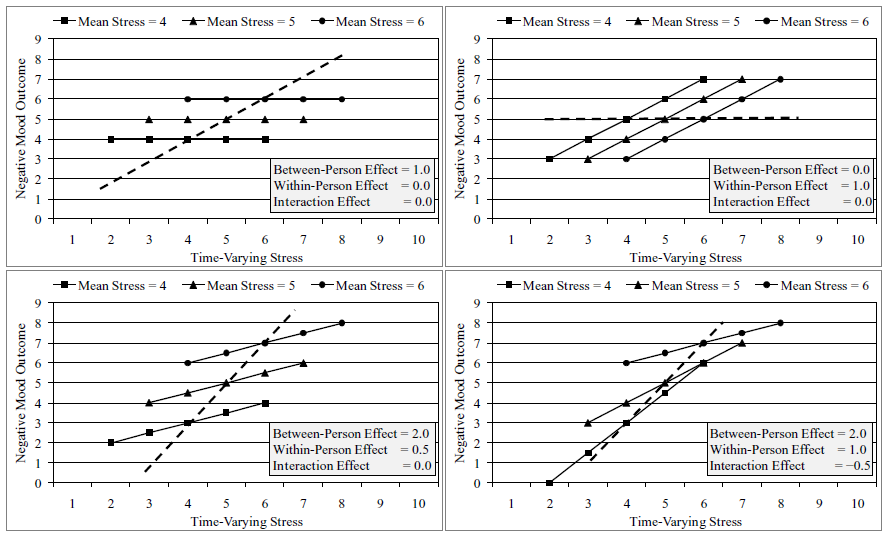
\includegraphics{img/lessa1.png}
	\caption{Efectos hipotéticos entre-persona (como la pendiente de la línea
	discontinua a través de la media de la persona) y efectos intra-persona
	(como la pendiente de la línea completa para la media = 5; marcadores
	triangulares) del estrés variable en el tiempo sobre el estado de ánimo
	negativo variable en el tiempo.}
	\label{lessa_1}
\end{figure}

Aquí el estrés y el estado de ánimo negativo son variables continuas con una
media de 5 para facilitar la explicación, y se trazan trayectorias separadas
para personas con una puntuación media de estrés a lo largo del tiempo de 4, 5
o 6. Nótese que el \textit{tiempo} no es necesario en \ref{lessa_1}: una vez
que se hayan incluido en el modelo los efectos fijos y aleatorios necesarios
relacionados con el tiempo, probablemente ya no importará en qué ocasión se
trate al considerar los efectos de CVT. Aquí, lo que necesitamos saber es cuál
fue el valor de estrés en cada ocasión, y no necesariamente \textit{cuándo} se
informó ese valor de estrés (sin embargo, en qué ocasión puede importar si el
efecto de la CVT cambia con el tiempo). Críticamente, tanto el estrés como el
estado de ánimo negativo tienen variación entre-persona y variación
intra-persona y, por lo tanto, existe la posibilidad de que el estrés muestre
un efecto tanto entre-persona como intra-persona, \ref{lessa_1} fue diseñado
para ilustrar diferentes patrones de estos efectos.

Para comenzar, el panel superior izquierdo de \ref{lessa_1} muestra un efecto
de estrés que es completamente \textit{entre-persona}: hay una pendiente
positiva de 1 a través de la media de estrés de la persona (como lo muestra la
línea discontinua a través de el centro de las trayectorias individuales), lo
que indica que por cada unidad mayor de \textit{estrés medio de la persona} se
espera que el estado de ánimo negativo medio sea superior a 1. O dicho de
manera más simple, las personas que reportan más estrés en promedio que otras
personas tienden a ser más gruñonas en promedio que otras personas. Sin
embargo, no hay efecto de estrés dentro de las personas (las trayectorias
individuales tienen una pendiente de 0), lo que indica que reportar \textit{más
estrés que su propia media} no tiene ningún efecto sobre el estado de ánimo
negativo de esa ocasión. Esto significa que el efecto del estrés en el panel
superior izquierdo es completamente \textit{transversal}: las diferencias
individuales en el estrés promedio a lo largo del tiempo se relacionan con el
estado de ánimo negativo promedio, pero la variación intraindividual en el
estrés no se relaciona con el estado de ánimo negativo de esa ocasión.

A continuación, considere el panel superior derecho de \ref{lessa_1}, que
muestra un efecto del estrés que es completamente \textit{intra-persona}: hay
una pendiente positiva de 1 en cada trayectoria de estrés individual, lo que
indica que para cada unidad \textit{más estrés que su propia media} (cualquiera
que sea su propia media), se espera que el estado de ánimo negativo de esa
ocasión sea 1 más alto. O dicho de manera más simple, se predice que el estado
de ánimo negativo será más alto de lo habitual en los días en que las personas
reportan más estrés de lo habitual. Sin embargo, esta vez no hay efecto del
estrés entre-persona: el estrés medio de la persona no predice el estado de
ánimo negativo medio de la persona. Entonces, el efecto del estrés en el panel
superior derecho es completamente \textit{longitudinal}: no es que las personas
crónicamente estresadas sean más gruñonas que otras personas, es que cada vez
que las personas reportan más estrés de lo normal (independientemente de lo que
sea ``habitua'', como lo indica el estrés medio de su persona), también son más
gruñones de lo habitual.

Sin embargo, rara vez encontramos solo un efecto entre-persona o solo un efecto
intra-persona de una CVT, es más probable que ambos efectos se observen hasta
cierto punto. Para ilustrar, considere el panel inferior izquierdo de
\ref{lessa_1}, que muestra los efectos de estrés positivos de ambos tipos. Pero
aquí el efecto entre-persona de 2 es mayor que el efecto intra-persona de 0.5:
la pendiente de la línea a través de las medias de las personas tiene una
pendiente de 1.5 más pronunciada que la pendiente de las trayectorias de estrés
individuales. En consecuencia, por cada unidad de \textit{estrés de una persona
sobre otras personas}, se espera que el estado de ánimo negativo sea 2 veces
más alto, pero por cada unidad de \textit{más estrés que la propia media}, se
espera que el estado de ánimo negativo de esa ocasión sea más alto en 0.5. Dada
la misma variabilidad tanto para el estrés como para el estado de ánimo
negativo (es decir, ICC de 0.5 para cada variable), este resultado significaría
que ser una persona más estresada (que otras personas) es más importante para
predecir el estado de ánimo negativo que tener una ocasión más estresante (de
lo habitual), pero aquí tanto las diferencias individuales como la variación
intraindividual en el estrés son importantes hasta cierto punto.

Hasta ahora, los efectos hipotéticos del estrés han sido aditivos en todos los
niveles, pero este no tiene por qué ser el caso. Para ilustrar, considere el
panel inferior derecho de \ref{lessa_1} en el que también está presente una
interacción entre el estrés entre-persona y el estrés intra-persona. En
consecuencia, los dos efectos principales del estrés ahora están condicionados
el uno al otro: el efecto de estrés entre-persona de 2 se aplica
\textit{específicamente cuando las personas están en sus propios niveles medios
de estrés} (p. ej., como lo muestra la línea discontinua a través de la estrés
medio de la persona), y el efecto de estrés intra-persona de 1 se aplica
\textit{específicamente para las personas en el valor central del estrés medio
de la persona} (p. ej., el estrés medio de la persona = 5 aquí, como lo indican
los triángulos). La interacción entre el estrés entre-persona y el estrés
intra-persona de -0.5 se puede interpretar de dos maneras equivalentes. Primero
(y más intuitivamente), significa que el \textit{efecto dentro-persona} de
reportar más estrés de lo habitual en una ocasión dada (que era 1 dado el
estrés medio de una persona = 5) \textit{se vuelve menos positivo por 0.5 por
cada unidad mayor del estrés medio de esa persona:} el efecto de reportar más
estrés de lo habitual importa \textit{menos} para las personas que tienen más
estrés en general. Alternativamente, la interacción entre el estrés
entre-persona y el estrés intra-persona de -0.5 también significa que el
\textit{efecto entre-persona} de reportar un mayor estrés medio que otras
personas (que es 2 cuando el estrés variable en el tiempo está en la media de
la persona) \textit{se vuelve menos positivo en 0.5 por cada unidad más de
estrés que lo habitual:} las diferencias entre las personas debido al estrés
medio son menos pronunciadas cuando las personas están más estresadas que lo
habitual.

Para resumir, es probable que las CVT sean informativas en múltiples niveles de
análisis porque casi siempre contienen variancia tanto entre-persona como
intra-persona, y es probable que cada fuente de variación tenga un efecto
diferente sobre el resultado. Estos efectos pueden ser aditivos o interactivos
(y cada uno de ellos también puede interactuar con otros predictores). La
experiencia sugiere que \textit{es la regla, más que la excepción, que los
efectos entre-persona e intra-persona de las CVT diferirán entre sí}, y hay (al
menos) dos razones para esto. La primera razón se relaciona con los constructos
teóricos medidos por la covariable en el análisis. En el ejemplo del estrés,
una confluencia de varios factores crónicos puede resultar en que un individuo
determinado sea una persona con "mucho estrés" o "bajo estrés", tales como
variables de personalidad, diferencias en el estilo de vida, etc. Sin embargo,
es probable que factores diferentes y más reales sean la razón por la que
algunos días son más estresantes que otros, como las desviaciones específicas
temporales de las rutinas normales de trabajo, familia o salud. Por lo tanto,
dado que la variación entre-personae intra-persona probablemente represente dos
constructos teóricos diferentes, su efecto sobre un resultado dado a menudo
será de diferentes magnitudes o incluso de diferentes direcciones. Pero además
de las diferencias en los constructos que reflejan, sin embargo, la segunda
razón por la cual los efectos entre-persona e intra-persona probablemente
difieran entre sí es simplemente porque son coeficientes no estandarizados. Es
decir, cantidades desiguales de variación entre-persona versus intra-persona
darán como resultado efectos fijos que se estiman en diferentes escalas
numéricas.

\subsection{El rol de las CVT en los modelos para la parte media}

Ahora consideramos los roles potenciales que pueden desempeñar las CVT en cada
parte del modelo. Se cree comúnmente que el papel de los efectos fijos de las
CVT en el modelo de las medias es aportar a la varianza residual intra-persona
($\sigma_e^2$). Si bien esto es cierto, no es toda la historia, porque los
predictores que varían en el tiempo deberán estar representados por dos
covariables separadas que distingan sus fuentes de variación entre-persona e
intra-persona para distinguir adecuadamente su potencial efecto entre-persona e
intra-persona en un resultado longitudinal. Por lo tanto, para ser más
específicos, es la parte \textit{intra-persona de la CVT} la que potencialmente
podría explicar la variancia $\sigma_e^2$ intra-persona. De manera similar, las
interacciones entre las partes intra-persona de dos o más CVT también
reducirían $\sigma_e^2$. En contraste, la parte \textit{entre personas de la
CVT} es en realidad una covariable \textit{invariante en el tiempo}. Y, como ua
sabemos, las covariables invariantes en el tiempo pueden modificar cualquier
término para la intersección, la asíntota, el cambio en el tiempo o el efecto
de cualquier CVT.

%%% NO ENTIENDO ESTO
% Al hacerlo, explican la variancia aleatoria de nivel 2 en el efecto de nivel
% 1 si el efecto de nivel 1 es aleatorio, o bien la varianza residual de nivel
% 1 si el efecto de nivel 1 no es aleatorio.

\subsection{El rol de las CVT en los modelos para la covariancia}

Además de los efectos fijos en el modelo de la parte media que pueden explicar
la variancia de la respuesta, una CVT puede contribuir al modelo de la
variancia de dos formas. Primero, los predictores variables en el tiempo pueden
tener \textit{efectos aleatorios}, es decir, cada persona puede necesitar su
propia pendiente para el efecto de la CVT. Por ejemplo, \textit{el efecto de
tener más estrés de lo normal} en el estado de ánimo negativo podría diferir
aleatoriamente entre las personas. Las diferencias individuales en las
pendientes se convertirían entonces en otra cantidad de variancia a predecir
(es decir, mediante interacciones entre niveles de la CVT con la pendiente
aleatoria con una o más covariables invariantes en el tiempo, tal como vimos en
secciones anteriores)

En segundo lugar, las CVT también se pueden usar para predecir la
heterogeneidad de la variancia en la respuesta. La \textit{parte entre-persona}
de una CVT puede predecir la heterogeneidad de la variancia entre persona (es
decir, cantidades diferenciales de las variancias de efectos aleatorios entre
personas) o la heterogeneidad de la variancia residual intra-persona (es decir,
cantidades diferenciales de fluctuación intra-persona entre personas). Pero la
\textit{parte intra-persona} de una CVT solo puede predecir la heterogeneidad
de la variancia residual intra-persona. En resumen, especificar y evaluar
correctamente las muchas contribuciones de una CVT (y todas sus partes aditivas
e interactivas) en un modelo longitudinal puede ser una tarea bastante
compleja.

%%%
% ACA IRIA EL CAPITULO 1.F DE LESSA HOFFMAN PERO NO LO ENTENDI
%%%

\section{Examinando los principales efectos multi-nivel de las CVT}

El ejemplo de este capítulo se basará en los mismos datos que se usaron
anteriormente. Se recopilaron cinco evaluaciones durante un período de dos
semanas de 105 adultos mayores de 69 a 95 años ($\hat{\mu} = 80.13,
\hat{\sigma} = 6.11$), el 27\% de los cuales eran hombres. La respuesta es la
suma de la cantidad de síntomas físicos que los participantes informaron haber
experimentado en las últimas 24 horas
($\hat{\mu} = 1.27, \hat{\sigma} = 1.32, rango posible = 0 a 5; ICC = 0.66$).
Un total de 509 casos estaban completos con respecto a las variables a incluir
(es decir, síntomas predichos por sexo, edad, estado de ánimo negativo diario y
estres diarios). Dado nuestro eventual interés en modelos con varianzas
heterogéneas, estimaremos todos los modelos utilizando la máxima verosimilitud
(ML). La significación los efectos fijos individuales se probará mediante sus
$p-value$ de prueba de Wald. La significación de un conjunto de múltiples
efectos fijos nuevos o de un nuevo efecto aleatorio se evaluará mediante
pruebas de razón de verosimilitud. Haremos las suposiciones habituales de
normalidad, así como independencia y variancia constante entre personas, días y
covariables.

% Lessa Hoffman terminado

\newpage
\nocite{*}
\renewcommand{\refname}{Bibliografía}
\bibliography{Bibliografia}

\end{document}